\begin{figure}[t]
\centering
\resizebox{\columnwidth}{!}{%
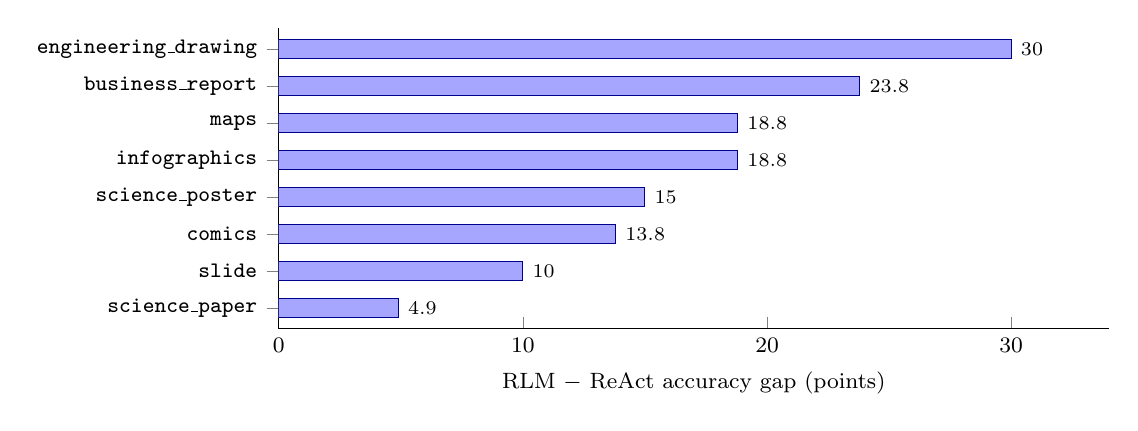
\begin{tikzpicture}
\begin{axis}[
  xbar, width=\columnwidth, height=5.4cm,
  bar width=7pt,
  enlarge y limits=0.08,
  xmin=0, xmax=34,
  xlabel={RLM $-$ ReAct accuracy gap (points)},
  xlabel style={font=\footnotesize},
  symbolic y coords={science\_paper,slide,comics,science\_poster,infographics,maps,business\_report,engineering\_drawing},
  ytick=data,
  yticklabel style={font=\footnotesize\ttfamily},
  xtick={0,10,20,30},
  tick label style={font=\footnotesize},
  nodes near coords, nodes near coords style={font=\scriptsize},
  nodes near coords align={horizontal},
  every node near coord/.append style={/pgf/number format/fixed,/pgf/number format/precision=1},
  axis x line*=bottom, axis y line*=left,
]
\addplot[draw=blue!55!black,fill=blue!35] coordinates {
  (4.9,science\_paper) (10.0,slide) (13.8,comics) (15.0,science\_poster)
  (18.8,infographics) (18.8,maps) (23.8,business\_report) (30.0,engineering\_drawing)
};
\end{axis}
\end{tikzpicture}%
}
\caption{The active-perception advantage tracks \textbf{visual density}. At matched perception (a shared 27B VLM, so the difference is purely harness), the RLM$-$ReAct accuracy gap by category is largest on detail-dense pages where cropping recovers fine structure (engineering drawings, business-report figures, maps, infographics) and smallest on text-linear ones (slides, scientific papers). Per-category cells are noisy (10 questions each); the ranking, not the exact value, is the point.}
\label{fig:category}
\end{figure}